% Marius: I think this part should establish a little more on the motivation and introduction part. Right now I think the reader has no idea what this is about if they were never exposed to the project before.


\subsection{Introduction}
\label{data-management-intro}
\textit{Author: Jacek Janczura}\\
Before diving into the details, we strongly believe that there is a need to  highlight the huge challenge that we faced during the early development process. 

Our greatest obstacle was the fact that the team had no access to the BMW's streaming data pipeline. The main reasons for that were the fact that this project was in an the early stage of development for BMW, as well as that fact that such a permission would pose a security threat to their team. Later, the BMW team provided only a small piece of an offline, aggregated data. More detailed explanation of how the data was handled will be presented in \textit{section \ref{data-processing-intro}}. The initial lack of data was the reason why the team had to be creative and try to find some work-arounds. We started the project by using some sample data found online and then after getting familiarised with the process of handling the data, we generated a mock of the streaming data, process explained in \textit{section \ref{sec:streaming-data-approach}}.\\
This way, the following section will presents not only the architecture of the final delivered product, but will also include temporary solutions that worked for the first development stages of the product. We insisted on presenting them to the reader, as they offered important expertise in data handling.

\subsection{High-level description of the pipeline architecture}
\label{sec:architecture_description}
\textit{Author: Jacek Janczura} \\
In the previous introductory section we talked about the faced "data issue". Due to this challenge, we decided that the best approach towards data would be to handle it in a parallel manner. We chose to divide our pipeline into two main sub-components, one dealing with \textbf{streaming data} and the other one with \textbf{offline data}.

\begin{itemize}
    \item \textbf{The Offline (or Fixed) approach}. Due to the lack of real time data streaming, we needed to prepare, test and train various machine learning models (DeepAR, RCF and Mean Predictor) for anomaly detection (RCF, Mean Predictor) and prediction (DeepAR, Mean Predictor, Holt-Winter's). At first, we conducted a research and picked the aforementioned models as the most promising ones.
    Then we deployed those models on AWS SageMaker to test them using faked data from the internet with some anomalies, as well as self generated data in a format of BMW data. As the models worked, we could export them as endpoints ready to be fed with real streaming data.
    
    \item \textbf{The Streaming data approach}. Streaming data part is a pipeline, which should receive real time data or a mock receiving real time data, preprocess it and feed ML models deployed as an AWS Sage Maker endpoints to detect the anomalies.
\end{itemize}

\begin{figure}[h]
    \centering
    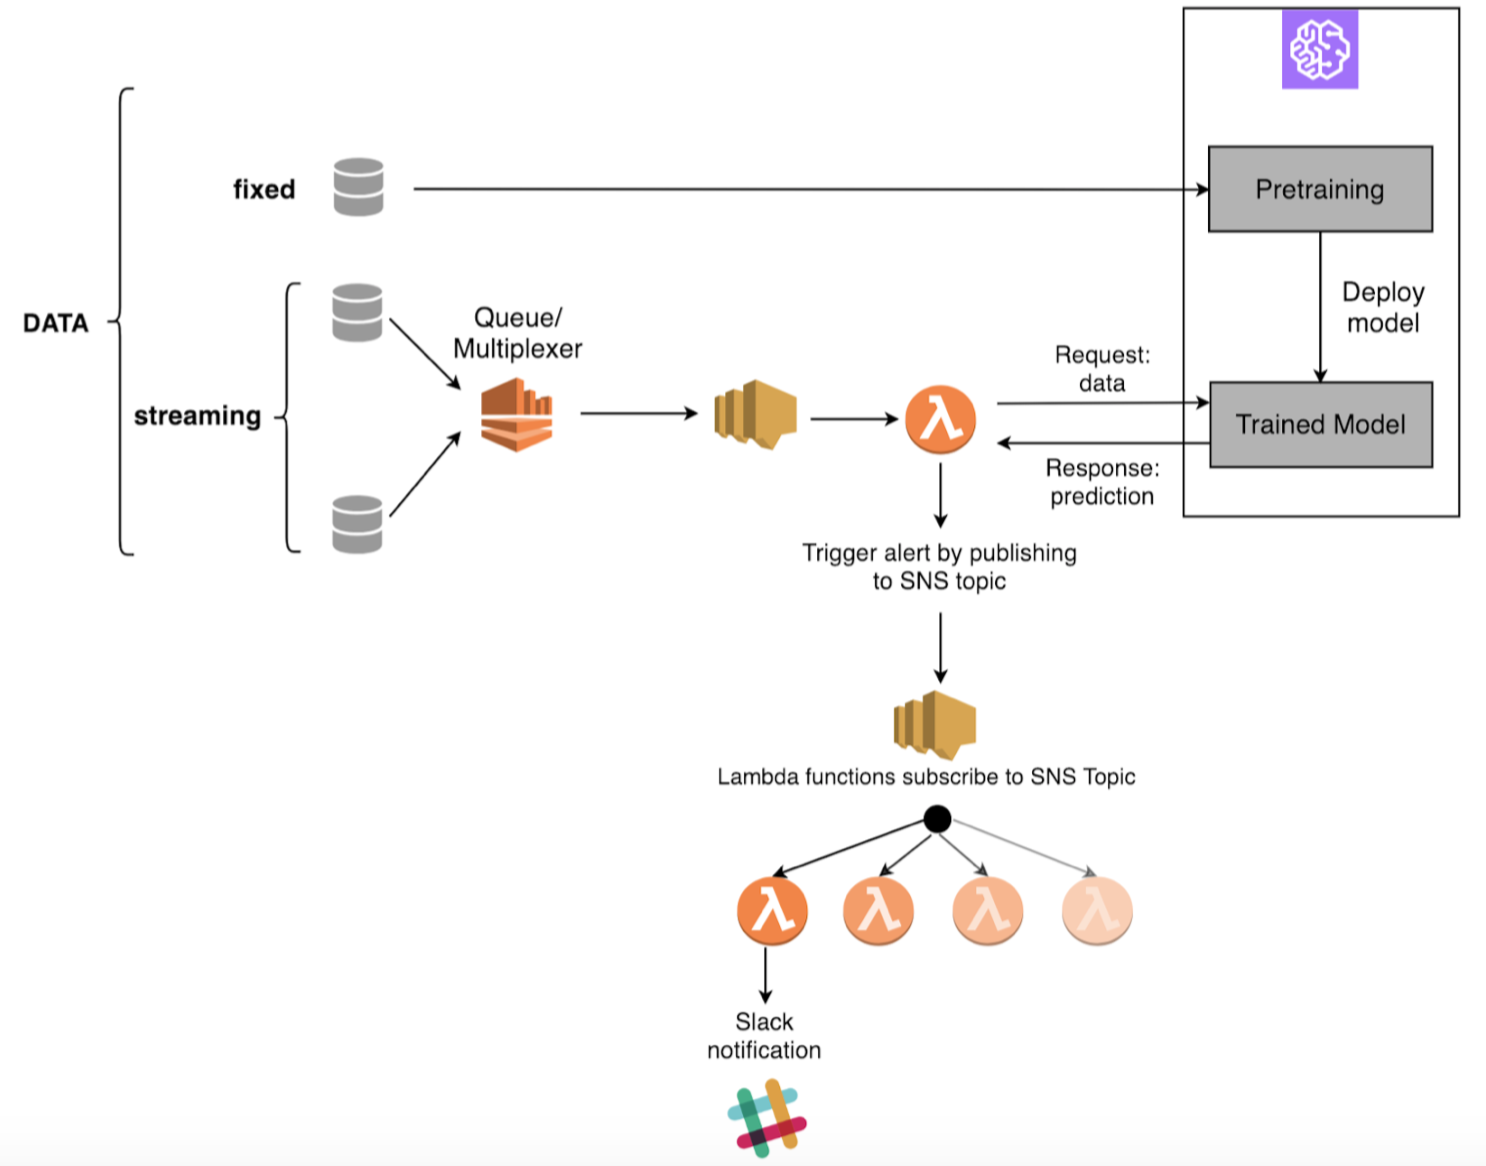
\includegraphics[width=1\textwidth]{images/sys-architecture.png}
    \caption{High-level system architecture, excluding Kinesis-based RCF pipeline}
    \label{fig:architecture}
\end{figure}
    
Let's explain those two approaches step by step, using the fig. \ref{fig:architecture}.\\ \textbf{Please note that this figure does not show the Kinesis-based RCF pipeline \ref{sec:streaming-data-approach}, which differs significantly from the example presented below (as it was developed independently). For more details regarding this particular pipeline, please read section \ref{sec:streaming-data-approach}.}
\begin{itemize}
    \item \textbf{Offline / Fixed}
    \begin{enumerate}
        \item Offline BMW's data resides into a specific S3 bucket, ready to use. It was provided in two forms: default flowlogs files and  preprocessed files (c.f. \lstinline{mock_data/output.json.example}).
        \item AWS Sagemaker \cite{awssagemaker} is used to train several machine learning models (DeepAR \cite{awsdeepar}, Mean Predictor [\ref{mean-predictor}] and Random Cut Forests \cite{awsRcf}) from the S3 bucket. It is also responsible for exporting them as endpoints, which implies that they are reachable via HTTP requests to run inferences.
    \end{enumerate}
    
    \item \textbf{Streaming}\\
    As explained in the previous section \ref{data-management-intro}, we built a system providing us with mock of streaming data that we aimed to process as if it was uploaded by the BMW pipeline.
    \begin{enumerate}
        
        \item The streaming data appears regularly in a specific (configurable) S3 bucket. 
        \item Each new batch of data arriving to this bucket triggers a new SNS Event \cite{awssns}, which on upload triggers AWS Lambda \cite{awslambda} functions. \\
        Those functions have diverse roles, but are in most cases used to contact our models exported as SageMaker endpoints. The models are the core elements containing the business logic of the project. They request our exported models for either anomaly detection or forecasting. 
        \item Finally, once the results are received, they are forwarded to either the \textbf{Chatbot API}, which calls the user to notify them about the anomalies and allows them to make an action, or to our own Slack channel, for real-time monitoring.
        
        
    \end{enumerate}
\end{itemize}
